\chapter{Network Measurements}
\label{chp:measurements2}

This chapter will display the experiments conducted on data sending rate from the nRF52 to the Raspberry Pi in the form of and graphs, tables and figures to try to determine the most efficient combination of amount of data to send, sending frequency as well as protocols to use. 

%\section{temp/notes}

%Trying to understand the details of a capture in Wireshark. 

%Can fragmentation give us an advangate, if you can send more data pr header. 

%An empty char array sent over CoAP is 76 bytes. 
%19 bytes char array, 96 bytes
%21 bytes char array, 98 bytes. Adds only as much as needed. 
 



\section{Packet fragmentation}

In Internet Routing, \textit{fragmentation} is known as the action of splitting data into smaller packets, to satisfy the maximal limits of the different technologies or protocols used (e.g. \gls{ble} and \gls{6lowpan} in the network described in this thesis). Each of these packets needs header fields of a certain size, or other requirements.

To better understand fragmentation, imagine a train with carriages as shown in Figure \ref{fig:trainExample}. To be able to operate at all, the train needs a locomotive with an engine driver, a conductor and a cafe carriage. As soon as these things are already there, the company owning the train gets better and better off for every passenger buying a ticket. Lets assume that every carriage can carry 4 employees and 27 passengers, to make it directly comparable to the \gls{ble} packets in the network. Eventually all the carriages will be full, and a decision has to be made if it will be profitable to fit another carriage. It will in general be most profitable to use as many carriages as the locomotive can handle, and to fill up every carriage as much as possible. It will however not be a good idea to connect another carriage if there will only be one additional passenger sitting there, since the extra weight of the carriage adds unnecessary additional weight to the train set compared to the income. 

\begin{figure}[ht]
    \centering
    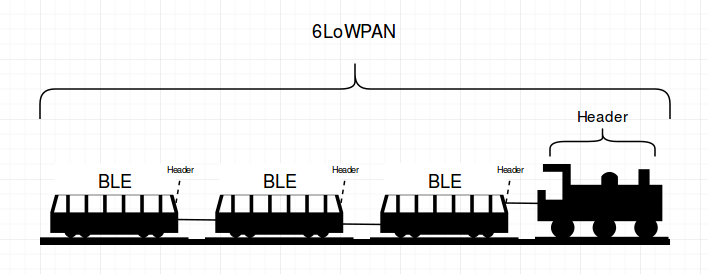
\includegraphics[scale=0.5]{trainExample.png}    
    \caption{Packet fragmentation - train comparison}
    \label{fig:trainExample}
\end{figure}

In this example, the locomotive and employees are the \gls{6lowpan} packet, that are needed no matter what to get the train working. Each additional carriage is a \gls{ble} packet. The goal is therefore to find the maximal number of passengers compared to the cost of adding additional carriages, in other words the maximal number of bytes compared to the number of packets sent. This is known as \textit{fragmentation}, to maximize \textit{goodput} vs \textit{throughput}. 


\section{CoAP NON}

When sending \gls{ble} packets over the network, observations from the system shows that the maximum packet size over \gls{ble} is 31 bytes. Each of these packages needs a header field of 4 bytes, meaning 27 bytes left for useful data. However, to start the connection at all, 76 byte is needed, meaning three \gls{ble} packets. The ratio between \textit{useful} and \textit{needed} (known as \textit{goodput} and \textit{throughput}) data transferred therefore start out very poorly if the payload sent is very small. 

Figure \ref{fig:goodputThroughputGraph} shows the correlation between goodput and throughput compared to the number of packets sent. In this particular case it makes no sense to send less than 50 bytes at once, since more than 50 \% of the data will be header files. This is comparable to have a locomotive and full crew at disposal, but only a few or none paying passengers. The best possible result is to have every carriage full, with 27 passengers and 4 employees. Since at least 4 bytes out of every 31 sent needs to be used to header information, the best possible result will be 87,1 \%. Mathematically, this is described as a \textit{horizontal asymptote} since the distance between the graph and \textit{y = 87,1} will approach zero after an infinite number of bytes has been transferred. The graph will therefore converge to 87,1 \%, just as shown in figure \ref{fig:goodputThroughputGraph}, even before packet size of 200 bytes.  


\begin{center}
 \begin{tabular}{||c c c c||} 
 \hline
 Goodput & Throughput & NON packet size & (Goodput/Throughput)*100 \\ [0.5ex] 
 \hline\hline
 0 & 71 & 76 & 0 \\ 
 \hline
 1 & 73 & 78 & 1,37 \\
 \hline
 10 & 82 & 87 & 12,20 \\
 \hline
 20 & 92 & 97 & 21,74 \\
  \hline
 30 & 75 & 107 & 30,0 \\
  \hline
 40 & 85 & 117 & 47,06 \\
  \hline
 50 & 99 & 127 & 50,51 \\
  \hline
 60 & 109 & 137 & 55,05 \\
  \hline
 70 & 119 & 147 & 58,82 \\
  \hline
 80 & 133 & 157 & 60,15 \\
  \hline
 90 & 143 & 167 & 62,94 \\
 \hline
 100 & 153 & 177 & 65,36 \\
 \hline
 110 & 167 & 187 & 65,87 \\
 \hline
 120 & 177 & 197 & 67,80 \\
 \hline
 130 & 191 & 207 & 68,06 \\
 \hline
 140 & 207 & 217 & 69,65 \\
 \hline
 150 & 211 & 227 & 71,09 \\
 \hline
 160 & 225 & 237 & 71,11 \\
 \hline
 170 & 235 & 247 & 72,34 \\
 \hline
 180 & 253 & 257 & 71,15 \\
 \hline
 190 & 263 & 267 & 72,24 \\
 \hline
 200 & 277 & 277 & 72,20 \\ [1ex] 
 \hline
\end{tabular}
\caption{Measurements, BLE, constant length}
\label{table:1}
\end{center}



\begin{figure}[ht]
    \centering
    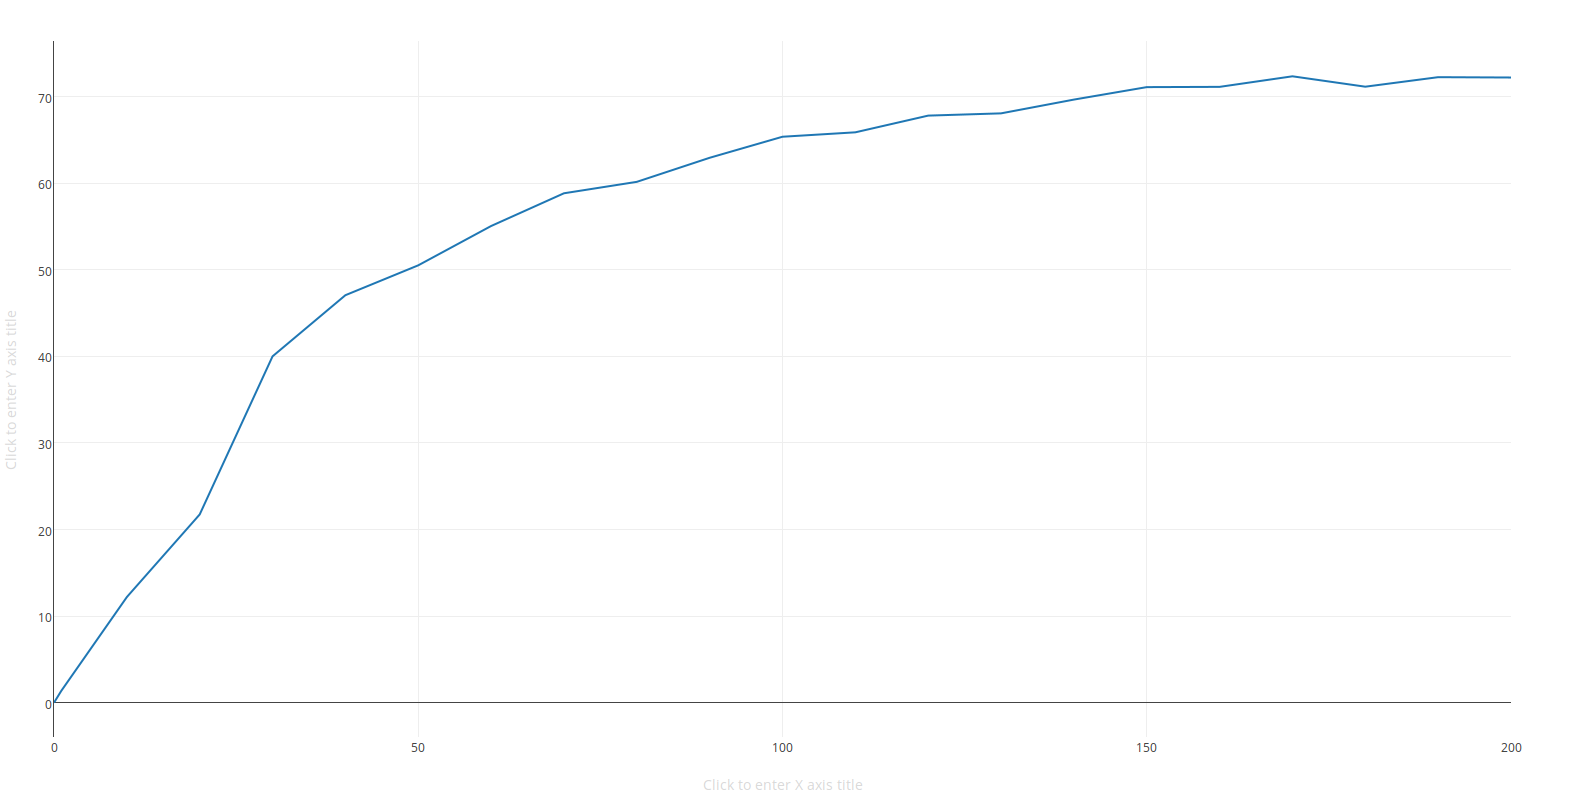
\includegraphics[scale=0.25]{graph1.png}    
    \caption{Goodput compared to throughput in \%}
    \label{fig:goodputThroughputGraph}
\end{figure}



\begin{figure}[ht]
    \centering
    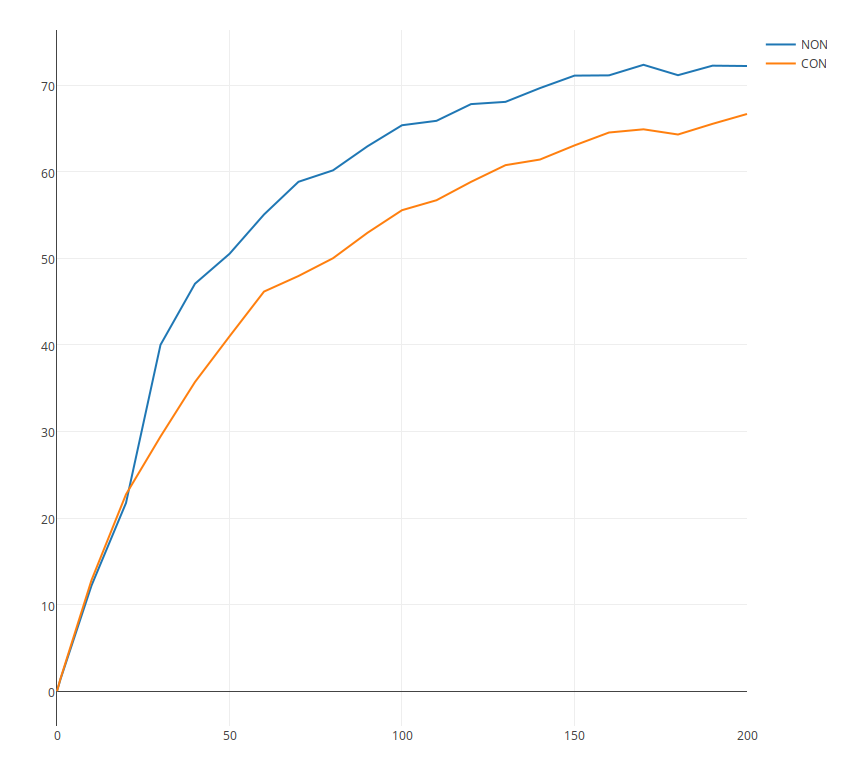
\includegraphics[scale=0.45]{CONvsNON1.png}    
    \caption{CON vs NON}
    \label{fig:CONvsNON}
\end{figure}


\begin{figure}[ht]
    \centering
    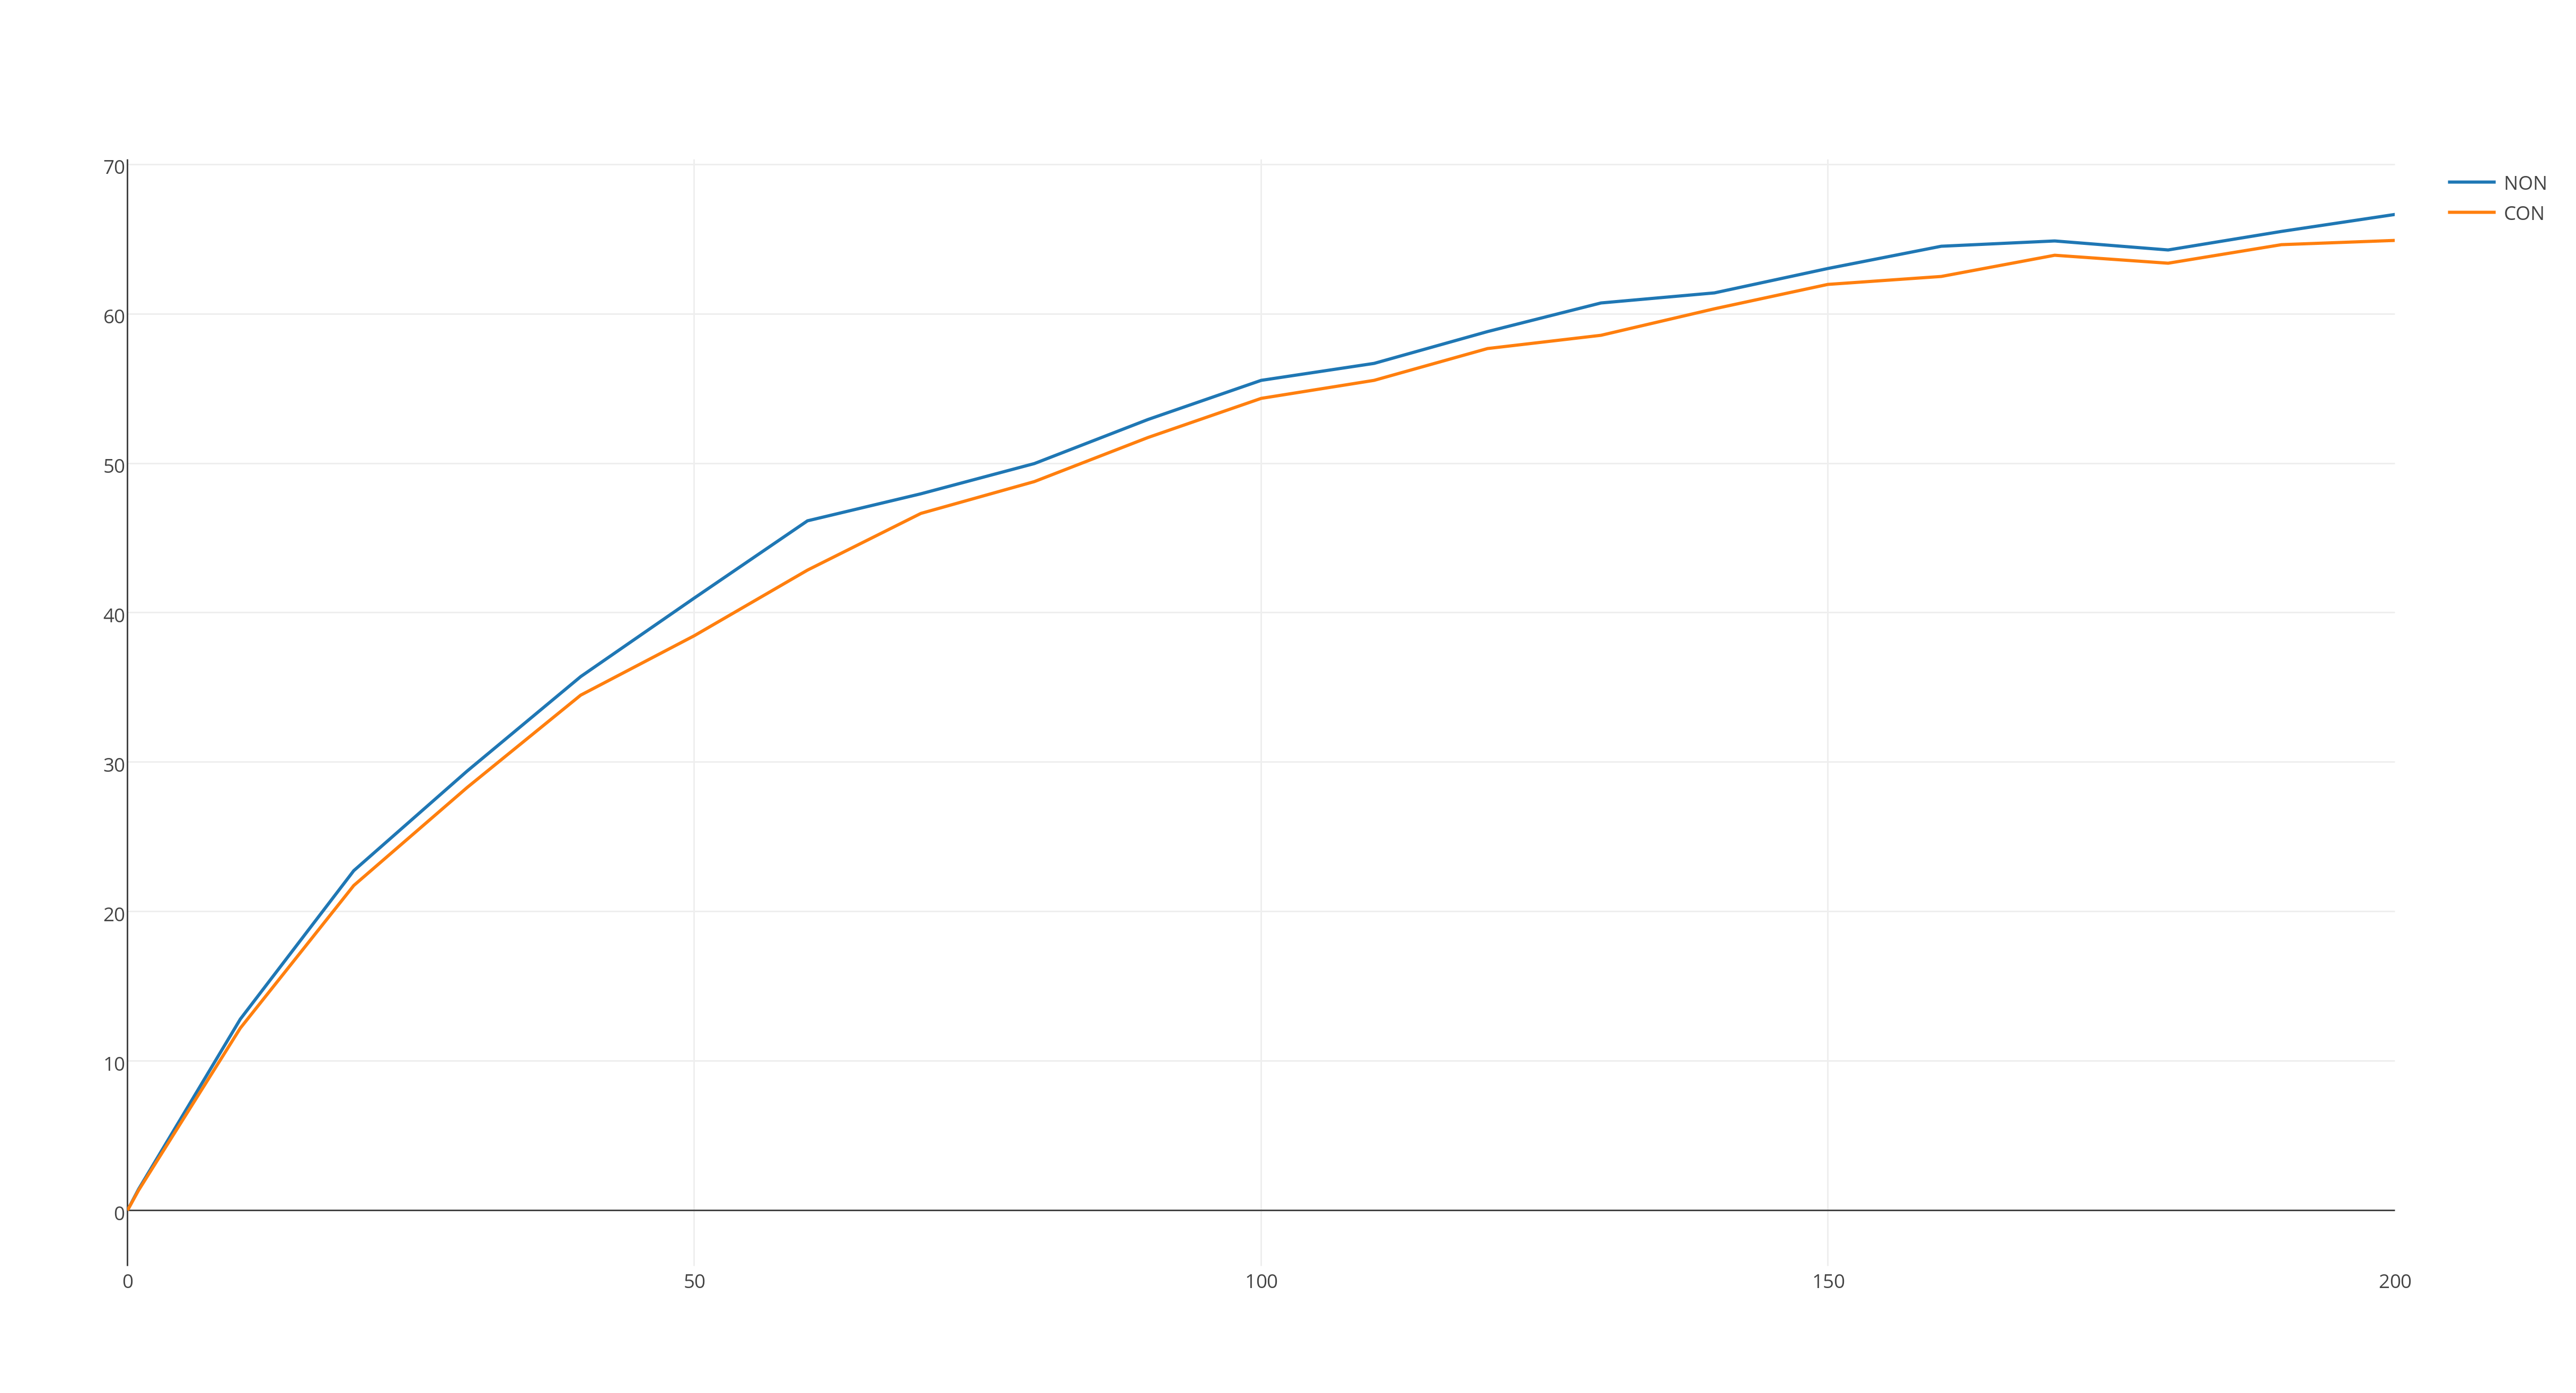
\includegraphics[scale=0.35]{NONvsCON_0-200.png}    
    \caption{CON vs NON 0-200 bytes}
    \label{fig:CONvsNON0-200}
\end{figure}


%\begin{figure}[ht]
%    \centering
%    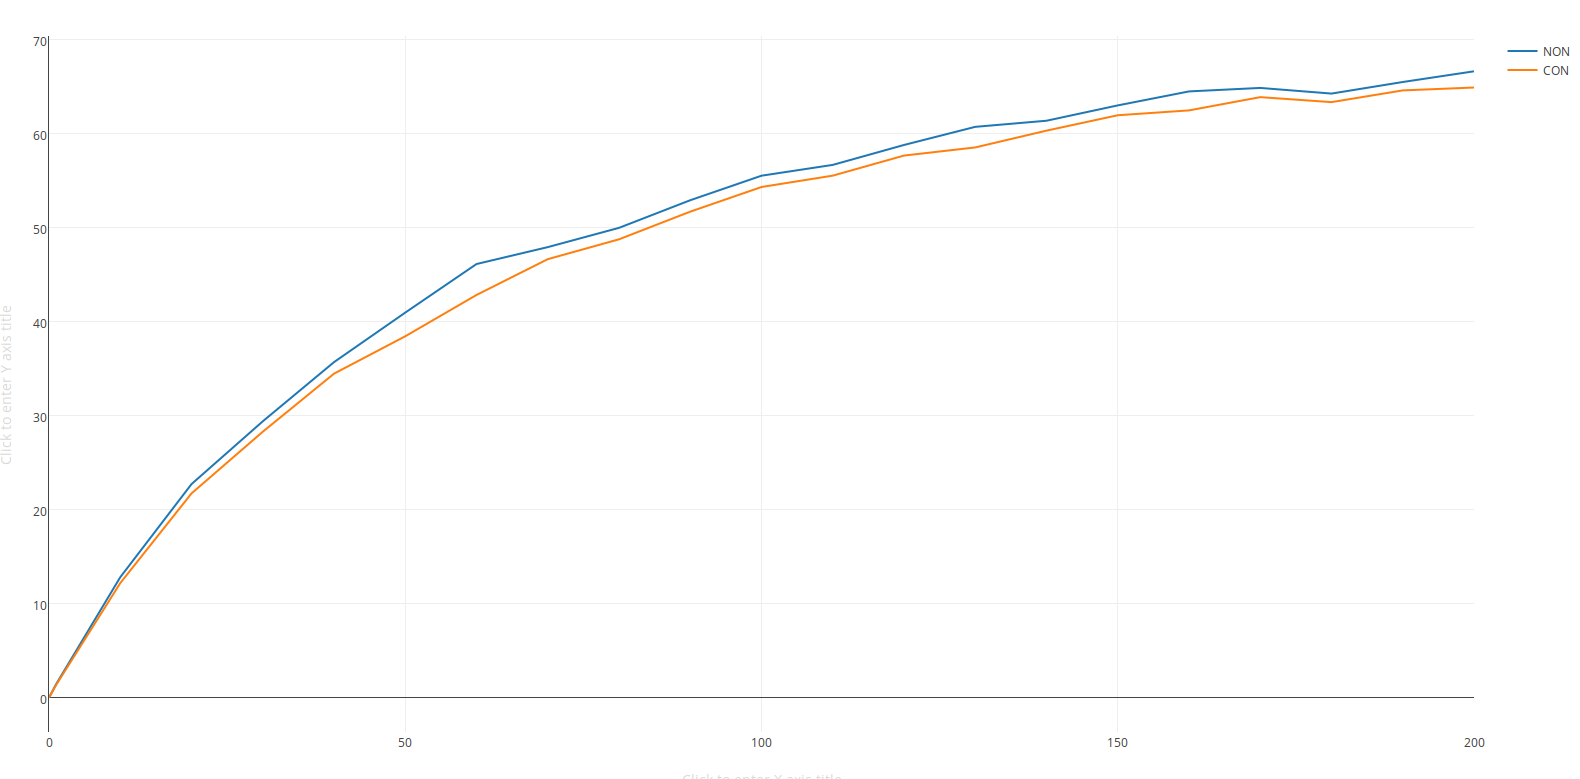
\includegraphics[scale=0.25]{CONvsNON0-200_2.png}    
%    \caption{CON vs NON 0-200 bytes number 2}
%    \label{fig:CONvsNON0-200}
%\end{figure}

\begin{figure}[ht]
    \centering
    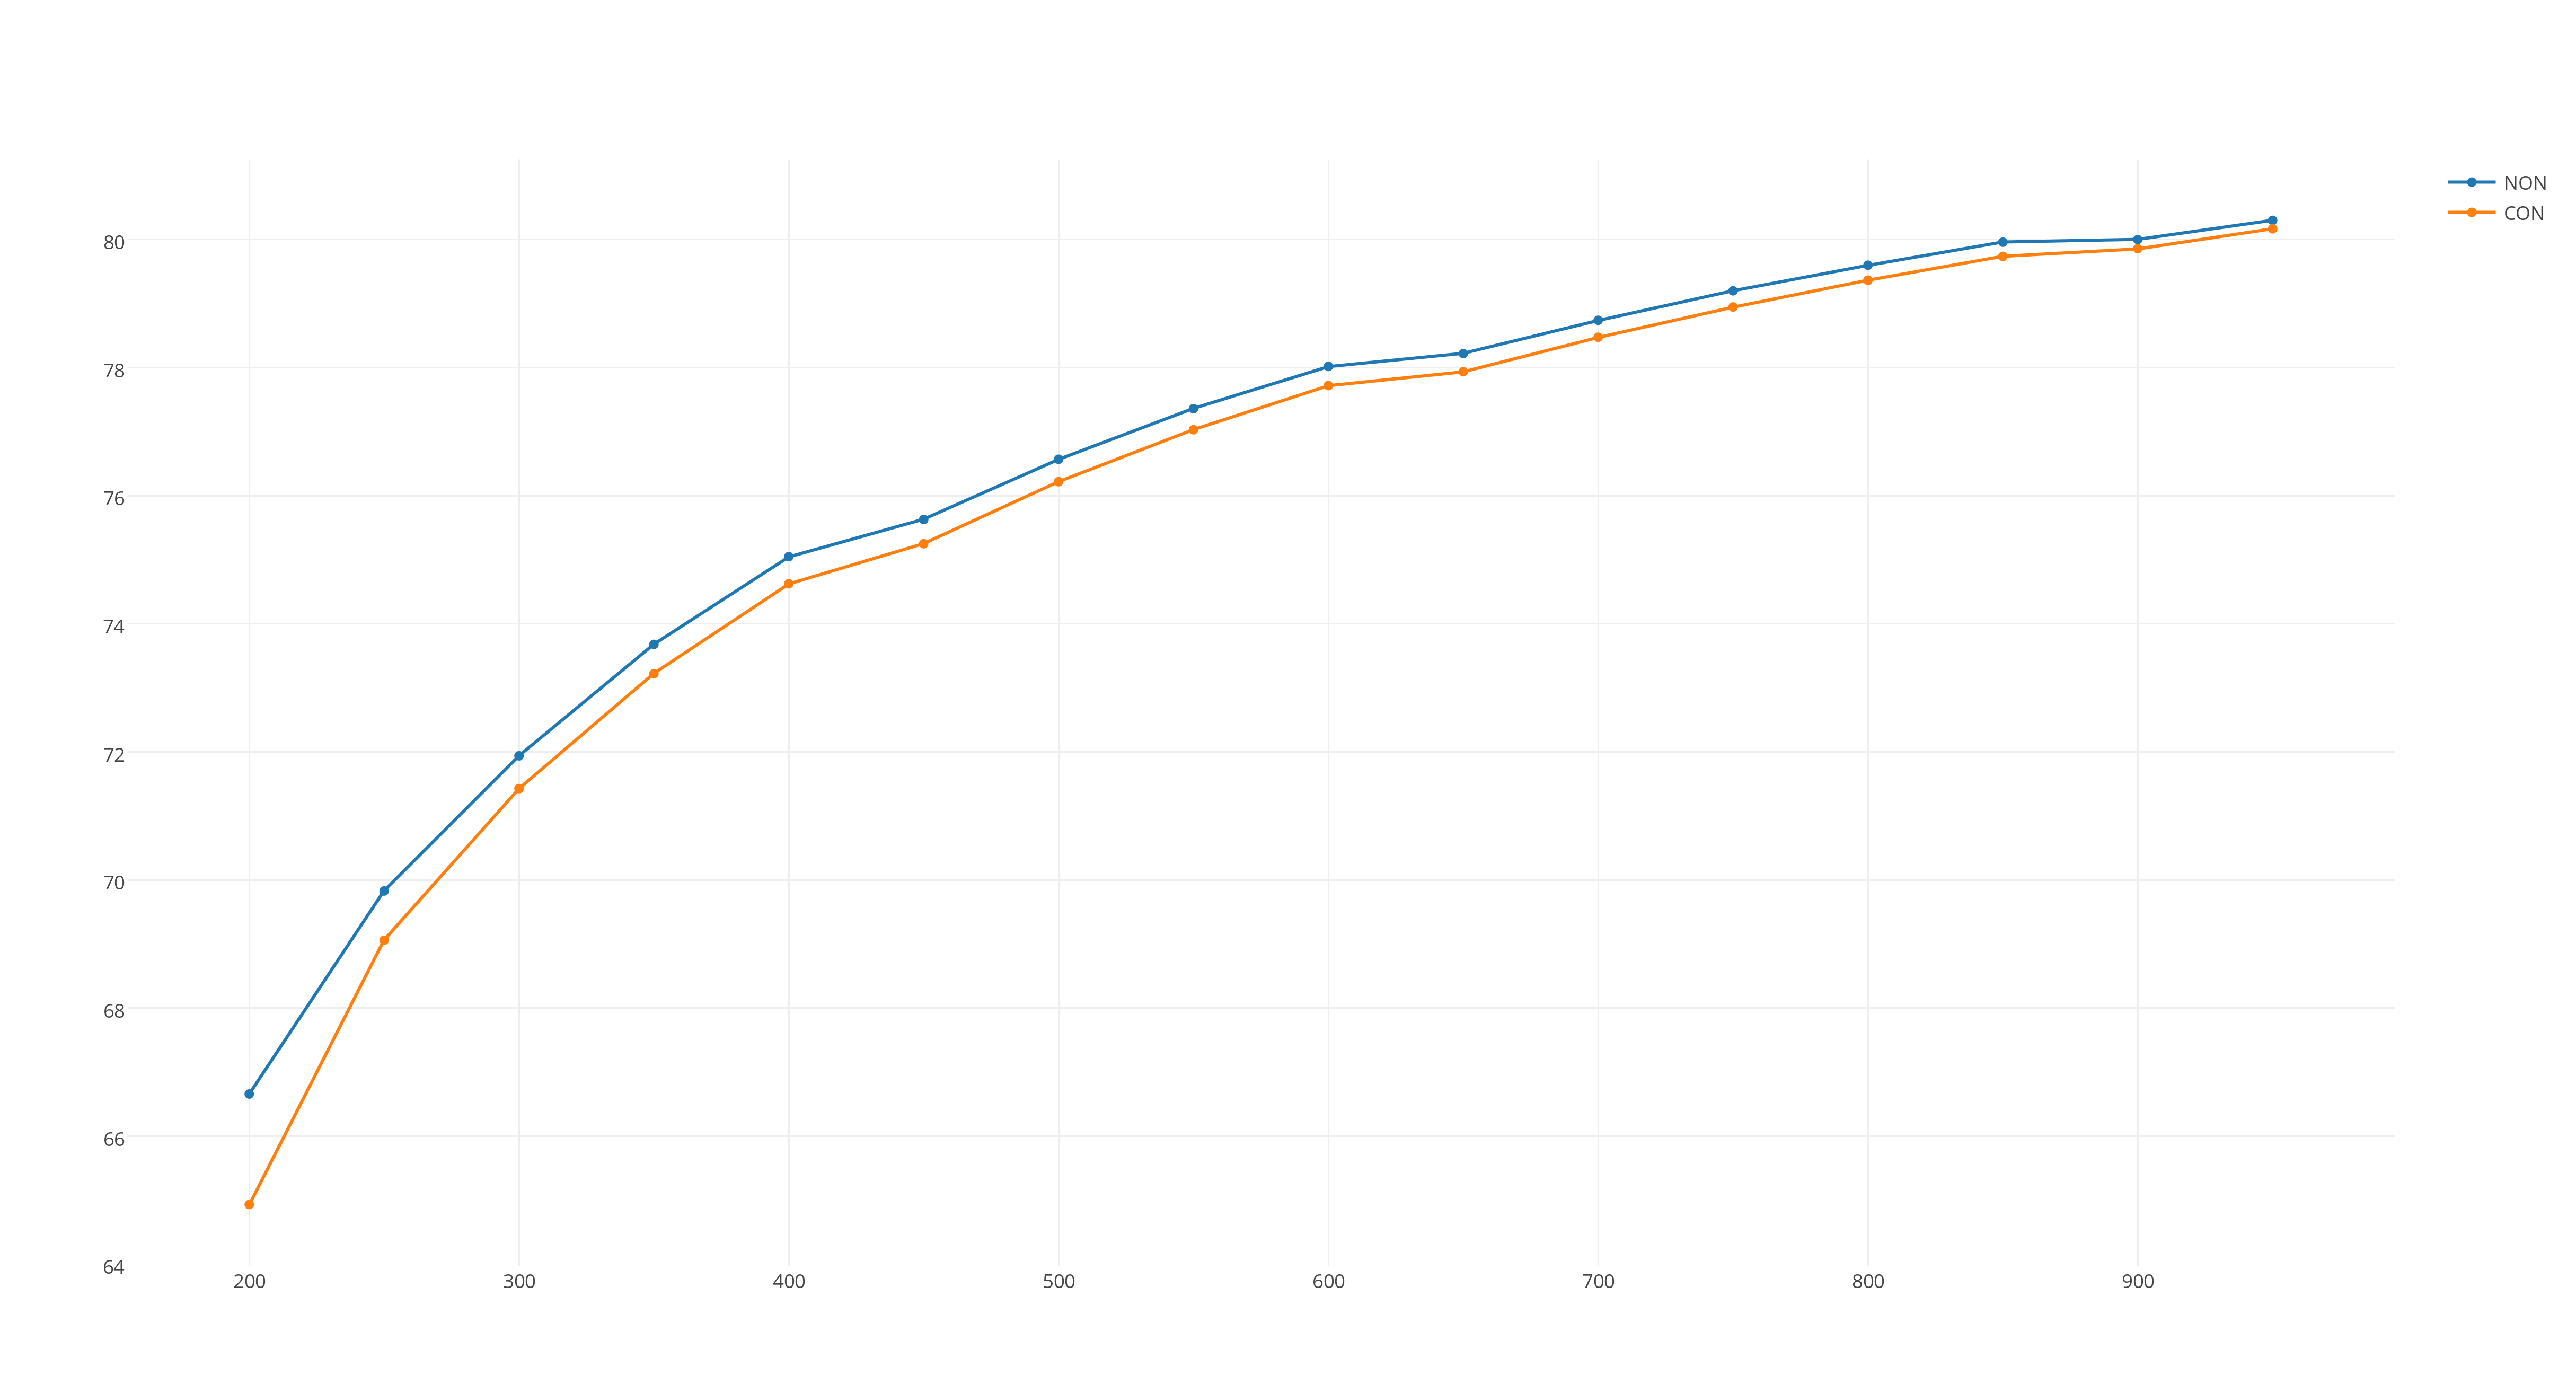
\includegraphics[scale=0.35]{NON-CON_200-950GRAPH.png}    
    \caption{CON vs NON 200-950 bytes}
    \label{fig:CONvsNON200-950}
\end{figure}




\subsection{Discussion}

Even though this first test was done with a very limited amount of data transferred, it is easy to see that the curve clearly flattens out to the asymptote of the graph at 87,1 \%. The next step would normally be to transfer a larger amount of data, just to verify that these assumptions are true. The limitations of transfer rate is not nearly yet met by either \gls{ble} or \gls{6lowpan}. This test will therefore be explained in the next section. 

However, given that there is already a clear limit in figure \ref{fig:goodputThroughputGraph} even before the transfer rate reached 200 bytes, way before expected, it also makes sense to test various other transfer protocols. If it is possible to find a way of transportation that could give a higher mathematical maximum, and also get to this limit faster, it would be very profitable to the transfer of goodput in the system. Because the stable transfer interval at the moment is once every second, it also makes sense to test \gls{coap} with \gls{ack} for every packet, \textit{CON} instead of \textit{NON}. Maybe this means that the header files can be smaller for each packet, and that the useful amount of data sent true therefore will be higher. 


\section{CoAP NON, with more data}

\subsection{Discussion}

\section{CoAP CON}

\subsection{Discussion}

\subsection{CoAP CON, with more data}

\subsection{Discussion}

